\documentclass[../../dissertation.tex]{subfiles}
\begin{document}

\subsection{Grover}
Like it was seen in section \ref{sec:chapGrover} Grover's algorithm is a tool that provides quadratic speedups to unstructured search problems. The routine consists on applying an oracle
\begin{equation}
        \mathcal{O}\ket{x} = (-1)^{f(x)}\ket{x},
\end{equation}\par
that flips the solution states, followed by an amplitude amplification process by means of the diffusion operator 
\begin{equation}
        %TODO: Decidir se mantenho os H's.
        \mathcal{D} = (2\ket{\Psi_0}\bra{\Psi_0} - I) = H^{\otimes n}(2\ket{0}\bra{0} - I)H^{\otimes n},
\end{equation}
where $\ket{\Psi_0}  = \frac{1}{\sqrt{N}}\sum_{x=0}^{N-1} \ket{x}$. The unitary operator that describes the algorithm will then be
\begin{equation}
        \mathcal{U} = \mathcal{D}\mathcal{O}.
\end{equation}
%TODO: Se calhar desenhar o circuito sem ser no qiskit onde e obvio que se aplicam as cenas varias vezes?
As was before mentioned, this evolution will be done several times, depending on the number of elements. Optimal probability of success finding a single solution will be reached after approximately $\sqrt{N}$ steps, and $\sqrt{\frac{N}{K}}$ for $K$ solutions. Consider the $3$ qubit case, where $N=8$, with $3$ iterations, as shown in figure \ref{fig:groverCircuitQistkit}.
\begin{figure}[!h]
	\centering
	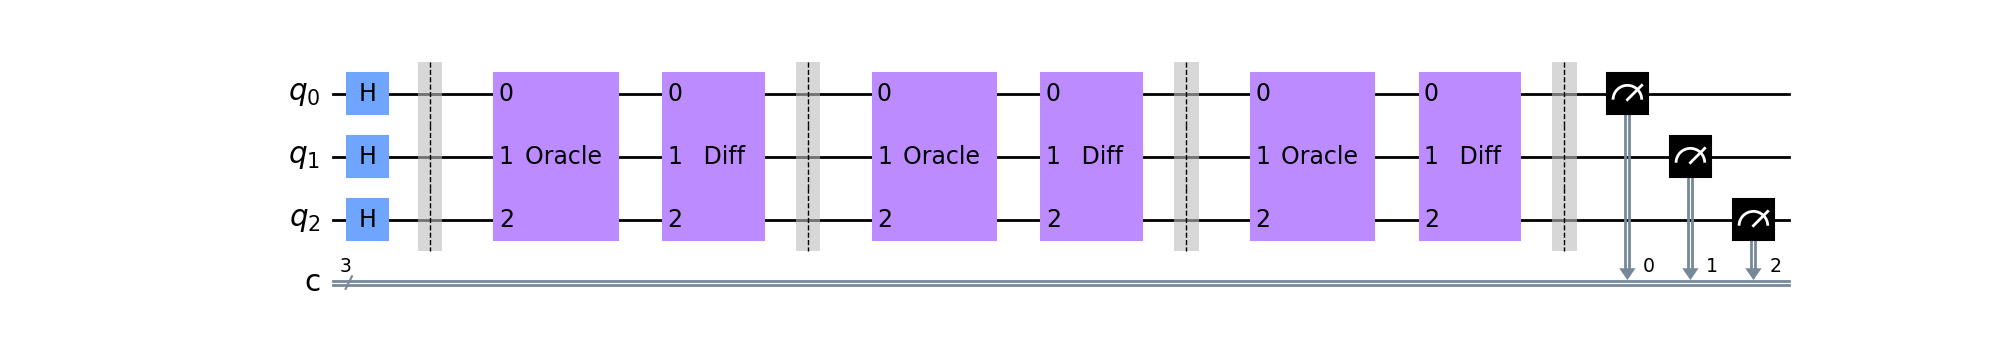
\includegraphics[scale=0.30]{img/Qiskit/GroverQiskit/Circuits/GroverQiskitCirc_N3_M4_S3.png}
	\caption{Temp}
	\label{fig:groverCircuitQistkit}
\end{figure}\par
%TODO: Escrever mais
The oracle circuit is shown in figure \ref{fig:groverOracleCircuitQistkit}. 
\begin{figure}[!h]
	\centering
	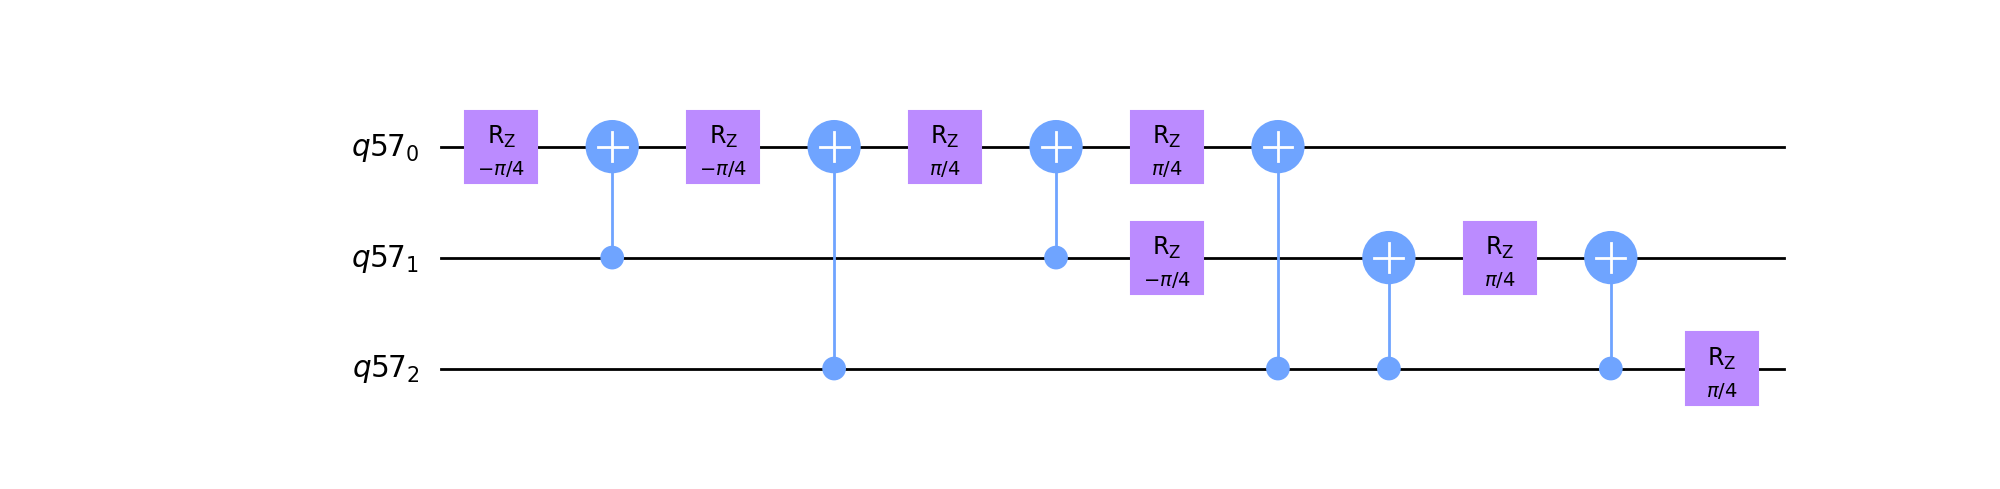
\includegraphics[scale=0.30]{img/Qiskit/GroverQiskit/Circuits/GroverQiskitCircOracle_N3_M4_S3.png}
	\caption{Temp}
	\label{fig:groverOracleCircuitQistkit}
\end{figure}\par
%TODO Escrever mais
The diffusion circuit is shown in figure \ref{fig:groverDiffCircuitQistkit}
\begin{figure}[!h]
	\centering
	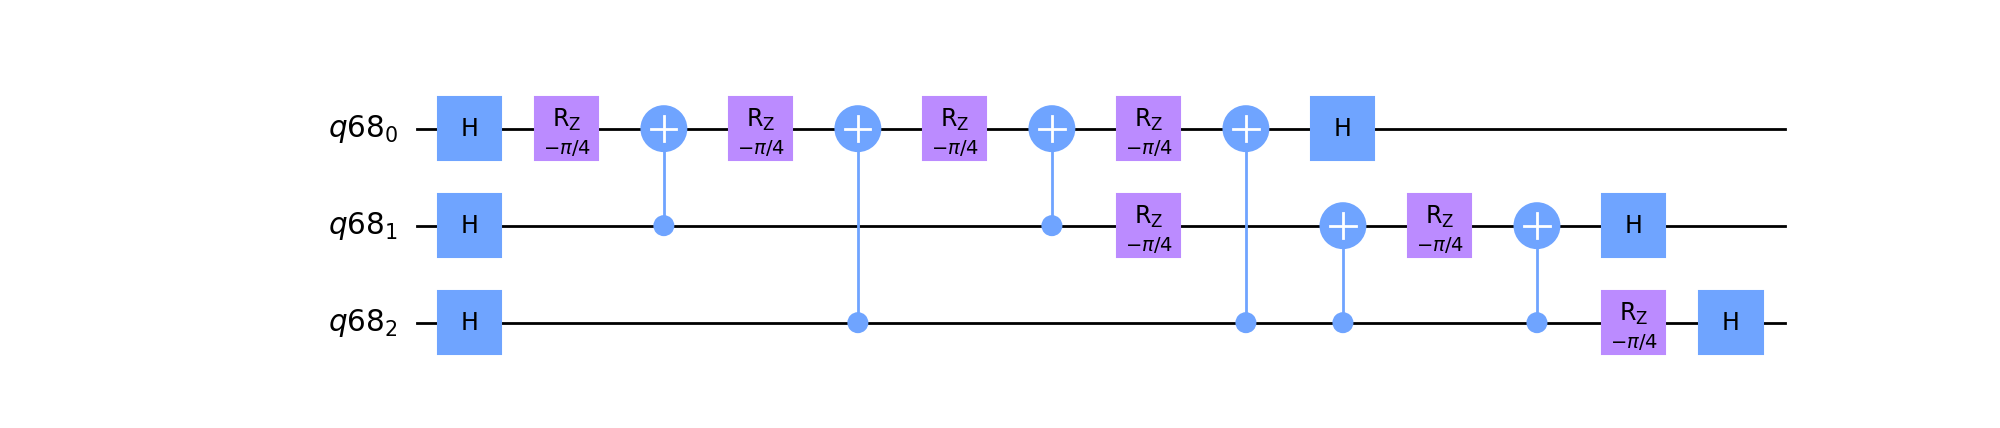
\includegraphics[scale=0.30]{img/Qiskit/GroverQiskit/Circuits/GroverQiskitCircDiff_N3_M4_S3.png}
	\caption{Temp}
	\label{fig:groverDiffCircuitQistkit}
\end{figure}\par
%TODO: Escrever mais
The results of measurement are shown in figure \ref{fig:groverQiskitDist}
\begin{figure}[!h]
	\centering
	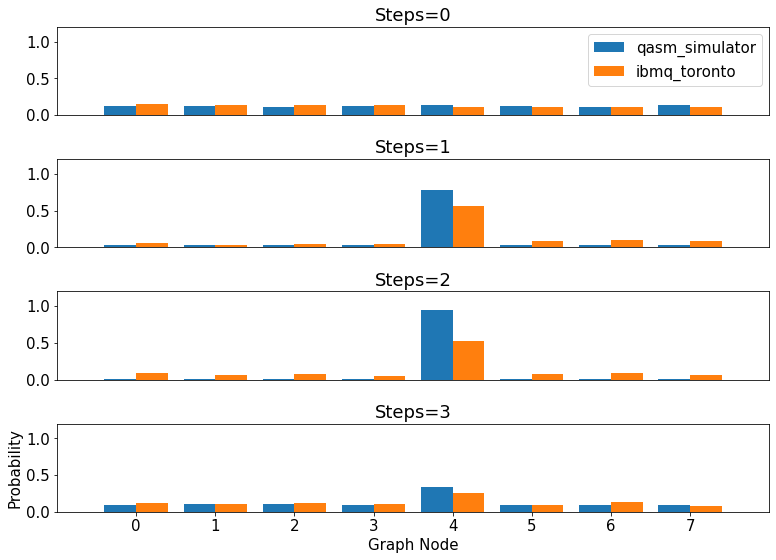
\includegraphics[scale=0.40]{img/Qiskit/GroverQiskit/GroverQiskitSearch_N3_M4_S0123}
	\caption{Temp}
	\label{fig:groverQiskitDist}
\end{figure}
%
\subsection{Coined}
%
%\begin{figure}[!h]
%	\centering
%	\includegraphics[scale=0.40]{img/Qiskit/CoinedQuantumWalk/Search/CoinedQiskitSearch_N4_M1_S01234}
%	\caption{Probability distribution for the staggered quantum walk on a line after 50 steps, with initial condition $\ket{\Psi(0)}=\frac{\ket{0}+\ket{1}}{\sqrt{2}}$, for multiple angles.} 
%	\label{fig:fig5}
%\end{figure}

%TODO: Fazer com outra moeda usando u3 com valores intermedios entre pi/2 ou pi/4
\subsection{Continuous}
\subsection{Staggered}

\end{document}
